\documentclass[a4paper, 15pt]{article}

\usepackage[margin = 1in]{geometry} % for spacing around
\usepackage{graphicx} % for including images in your pdfs
\usepackage{xcolor} % for including colors in your pdf
\usepackage{soul} % for text decoration
\usepackage[utf8]{inputenc} % for encoded text
\usepackage[T1]{fontenc}
\usepackage{setspace} % for setting different line spacings between paragrafs.
\usepackage{enumerate} % for letting us get more detailed enumerate lists
\usepackage{multirow} % to let us combine more rows together
\usepackage{colortbl} % for decorating tables
\usepackage{amsmath} % used for representing more complicated math displays
\usepackage{supertabular}
\usepackage{longtable} % both of these packages are used to making really big tables
\usepackage{wrapfig} % allows us to wrap text around figures
\usepackage{fancyhdr} % for making fancy headers
%\usepackage{bibtex} % for making better bibliographies
\usepackage[pdftex]{hyperref} % for letting us make links
\usepackage{lscape} % Allows us to flip from portrait to landspace
\usepackage{tikz} % for high detailed drawing
\usepackage{multicol} % To put things side by side
\usepackage{rotating} % For rotating objects
% \usepackage{draftwatermark} % For adding watermarks
\usepackage{MnSymbol} % for using multiple symbols
\usepackage{mathtools} % Used for more math symbols
\usepackage{xfrac} % For more complciated fractions and to add derivitives
\usepackage{hyperref} % for hyper links
\usepackage{enumitem} % for better enum lists
\usepackage{tcolorbox} % for adding colored text boxes
\usepackage{bm} % Adding bold text to math inputs

% Setting up the default image path
\graphicspath{{./Images/}}

% Implementing authro details
\title{Math 100 Cheat Sheet}
\author{Emre Arapcic-Uvak}
\date{}

% Setting up the fancy page style
\fancypagestyle{customStyle}{
	\lhead{} \chead{} \rhead{}
	\lfoot{} \cfoot{\thepage} \rfoot{}
	\renewcommand{\headrulewidth}{0pt}
	\renewcommand{\footrulewidth}{1pt}
}
\pagestyle{customStyle}

% Setting up hyperref options
\hypersetup {
	colorlinks = false,
	citecolor = black,
	filecolor = blue,
	linkcolor = blue,
	urlcolor = blue,
	pdftex
}

% Custom commands
\newcommand{\importantStar}{
	\begin{Large}
		\textcolor{red}{$\filledstar$}
	\end{Large}
}
\newcommand{\degC}[1]{
	$#1^\circ$
} 

% Custom colors
\definecolor{customOlive}{RGB}{207, 218, 166}

\begin{document}
	\maketitle
	\vspace{5mm}
	
	\begin{abstract}
		\begin{center}
			\noindent This document contains a set of identities and equations for Math100
		\end{center}
	\end{abstract}
	\pagebreak
	
	\tableofcontents
	\pagebreak
	
	\section{Logarithms}
		\subsection{General definition of a logarithm}
			\noindent Logarithms are inverse function of exponential function meaning that if we want to remove an exponent we can apply an logarithm
			
			\begin{equation*}
				\log_{b}(a) = c \implies b^c = a
			\end{equation*}
		
			\subsubsection{Example}
				\noindent Lets say that we want to figure out 2 to the power of what number gives us 524288, or in other words $2^x = 524288$. Well we can approach this problem in two ways, the first way is to apply the definition of the logarithm and phase the problem as such $x = \log_{2}(524288)$. Or we can do this by placing the both sides of the equation into logarithms as follows $\log_{2}(2^x) = \log_{2}(524288) \implies x = \log_{2}(524288)$.
				
				
			\subsubsection{Domain}
				\[\log_{b}(a) = c\]
				\noindent The logarithm above is valid for the following values:
				\[a \in (0, +\infty)\]
				\[b \in (0,1) \cup (1, +\infty)\]
		\subsection{Logarithm Terminology}
			\noindent These are some essential logarithm terminologies that can be found in many math books:
			\begin{enumerate}
				\item $\ln(a) = \log_{e}(a)$
				\item $\log(a) = \log_{10}(a)$
			\end{enumerate}
		\subsection{Logarithm Rules}
			\noindent There are a lot of rules that can help us when we are dealing with logarithms, some of these rules are:
			\begin{enumerate}
				\item $\log_{b}(1) = 0$
				\item $\log_{b}(b) = 1$
				\item $\log_{b}(b^x) = x$
				\item $\log_{b}(a^c) = c*\log_{b}(a)$
				\item $\log_{b}(a) + \log_{b}(c) = \log_{b}(a*c)$ \hspace{4mm} \importantStar
				\item $\log_{b}(a) - \log_{b}(c) = \log_{b}(\frac{a}{c})$ \hspace{4mm} \importantStar
				\item $\log_{b}(a) = \frac{\log_{c}(a)}{\log_{c}(b)}$ \hspace{4mm} \importantStar
			\end{enumerate}
		\pagebreak
		
	\section{Trigonometry}
		\subsection{Converting degrees into radians}
			\noindent If we mark the angle in degrees as \emph{$\alpha_{deg}$} and angle in radians as \emph{$\alpha_{rad}$}, the conversion goes as follows:
			\begin{equation*}
				\alpha_{rad} = \frac{\pi}{180^{\circ}} * \alpha_{deg}
			\end{equation*}
		
		\subsection{Converting radians into degrees}
			\noindent Same principal as before just our equation is now:
			\begin{equation*}
				\alpha_{deg} = \frac{180^{\circ}}{\pi} * \alpha_{rad}
			\end{equation*}
		
		\subsection{General definition of trigonometric functions}
			\noindent The concept of unit circle helps us to measure the angles of cos, sin and tan directly since the center of the circle is located at the origin and radius is 1. Consider $\theta$  to be an angle then
			
			\begin{figure}[h]
				\centering
				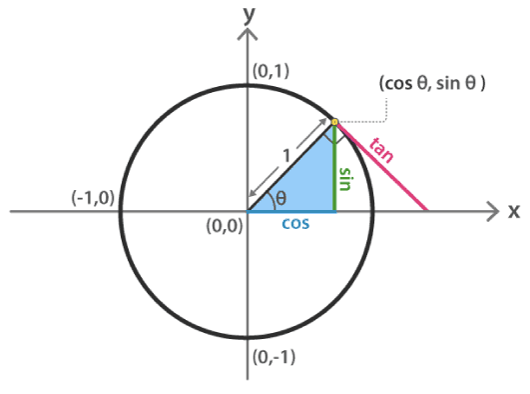
\includegraphics[width = .6\textwidth]{trigUnitCircle}
				\caption{Image of a trigonometric unit circle}
				\label{Fig:Trig Unit Circle}
			\end{figure}
		
		\subsection{Table of trigonometric values}
			{
				\centering
				\begin{tabular}{|c|c|c|c|c|c|c|c|c|}
					\hline \rowcolor{customOlive}
					$\alpha_{deg}$ & \degC{0} & \degC{30} & \degC{45} & \degC{60} & \degC{90} & \degC{180} & \degC{270} & \degC{360} \\ \hline
					$\alpha_{rad}$ & 0 & $\frac{\pi}{6}$ & $\frac{\pi}{4}$ & $\frac{\pi}{3}$ & $\frac{\pi}{2}$ & $\pi$ & $\frac{3\pi}{2}$ & $2\pi$ \\ \hline
					$\sin(\alpha)$ & 0 & $\frac{1}{2}$ & $\frac{1}{\sqrt{2}}$ & $\frac{\sqrt{3}}{2}$ & 1 & 0 & -1 & 0 \\ \hline
					$\cos(\alpha)$ & 1 & $\frac{\sqrt{3}}{2}$ & $\frac{1}{\sqrt{2}}$ & $\frac{1}{2}$  & 0 & -1 & 0 & 1 \\ \hline
					$\tan(\alpha)$ & 0 & $\frac{1}{\sqrt{3}}$ & 1 & $\sqrt{3}$ & \textcolor{red}{X} & 0 & \textcolor{red}{X} & 0 \\ \hline
				\end{tabular}
				\par
			}
		\pagebreak
	

		\subsection{Trigonometric Identities}
			\subsubsection{Trigonometry basis}
				\begin{itemize}
					\item $\tan(\theta) = \frac{\sin(\theta)}{\cos(\theta)}$
					\item $\cot(\theta) = \frac{\cos(\theta)}{\sin(\theta)}$
					\item $\tan(\theta) = \frac{1}{\cot(\theta)}$
					\item $\cot(\theta) = \frac{1}{\tan(\theta)}$
					\item $\sec(\theta) = \frac{1}{\cos(\theta)}$
					\item $\csc(\theta) = \frac{1}{\sin\theta)}$
				\end{itemize}
			\subsubsection{Pythagorean Identities}
				\begin{itemize}
					\item $\sin^2(\theta) + \cos^2(\theta) = 1$
					\item $\tan^2(\theta) + 1 = \sec^2(\theta)$
					\item $\cot^2(\theta) + 1 = \csc^2(\theta)$
				\end{itemize}

			\subsubsection{Reflections}
				\begin{itemize}
					\item $\sin(-\theta) = -\sin(\theta)$
					\item $\cos(-\theta) = \cos(\theta)$
					\item $\tan(-\theta) = -\tan(\theta)$
					\item $\cot(-\theta) = -\cot(\theta)$
					\item $\sec(-\theta) = \sec(\theta)$
					\item $\csc(-\theta) =  -\csc(\theta)$ 
				\end{itemize}

			\subsubsection{Angle Sum and Difference}
				\begin{itemize}
					\item $\sin(\alpha \pm \beta) = \sin(\alpha)\cos(\beta) \pm \sin(\beta)\cos(\alpha)$
					\item $\cos(\alpha \pm \beta) = \cos(\alpha)\cos(\beta) \mp \sin(\alpha)\sin(\beta)$
					\item $\tan(\alpha \pm \beta) = \frac{\tan(\alpha) \pm \tan(\beta)}{1 \mp \tan(\alpha)\tan(\beta)}$ 
					\item $\cot(\alpha \pm \beta) = \frac{\cot(\alpha)\cot(\beta) \mp 1}{\cot(\alpha) \pm \cot(\beta)}$
				\end{itemize}

			\subsubsection{Double Angle}
				\begin{itemize}
					\item $\sin(2\theta) = 2\sin(\theta)\cos(\theta)$
					\item $\cos(2\theta) = \cos^2(\theta) - \sin^2(\theta)$
					\item $\tan(2\theta) = \frac{2\tan(\theta)}{1-\tan^2(\theta)}$
					\item $\cot(2\theta) = \frac{\cot^2(\theta) - 1}{2\cot(\theta)}$
					\item $\sec(2\theta) = \frac{\sec^2(\theta)}{2-\sec^2(\theta)}$
					\item $\csc(2\theta) = \frac{\sec(\theta)csc(\theta)}{2}$
				\end{itemize}
			\subsubsection{Half Angle}
				\begin{itemize}
					\item $\sin(\frac{\theta}{2}) = \pm \sqrt{\frac{1-\cos(\theta)}{2}}$
					\item $\cos(\frac{\theta}{2}) = \pm  \sqrt{\frac{1+\cos(\theta)}{2}}$
					\item $\tan(\frac{\theta}{2}) = \frac{1-\cos(\theta)}{\sin(\theta)}$
				\end{itemize}	
\end{document}
